\documentclass[11pt]{article}
\usepackage[margin=0.92in,headheight=22pt]{geometry}
\usepackage{amsmath,amssymb,amsthm,bm,mathtools}
\usepackage{algorithm}
\usepackage{algpseudocode}
\usepackage{booktabs,tabularx,array}
\usepackage{graphicx}
\usepackage{pgfplots}
\pgfplotsset{compat=1.18}
\usepackage{xcolor}
\usepackage{enumitem}
\usepackage{fancyhdr}
\usepackage{microtype}
\usepackage{hyperref}

\definecolor{ink}{HTML}{172126}
\definecolor{teal}{HTML}{087E8B}
\definecolor{rust}{HTML}{C45A35}
\definecolor{soft}{HTML}{F3F6F5}
\definecolor{line}{HTML}{D5DEDB}

\hypersetup{
  colorlinks=true,
  linkcolor=teal,
  citecolor=teal,
  urlcolor=teal,
  pdftitle={MoEJointQuant: Modeling, Guarantees, and Staged Verification},
  pdfauthor={Method and verification note}
}

\pagestyle{fancy}
\fancyhf{}
\fancyhead[L]{\small\color{ink}MoEJointQuant}
\fancyhead[R]{\small\color{ink}Modeling and staged verification}
\fancyfoot[C]{\small\color{ink}\thepage}
\renewcommand{\headrulewidth}{0.4pt}
\renewcommand{\headrule}{\hbox to\headwidth{\color{line}\leaders\hrule height \headrulewidth\hfill}}

\theoremstyle{plain}
\newtheorem{theorem}{Theorem}
\newtheorem{proposition}{Proposition}
\newtheorem{lemma}{Lemma}
\newtheorem{corollary}{Corollary}
\theoremstyle{definition}
\newtheorem{definition}{Definition}
\newtheorem{assumption}{Assumption}
\theoremstyle{remark}
\newtheorem{remark}{Remark}

\newcommand{\R}{\mathbb{R}}
\newcommand{\E}{\mathbb{E}}
\newcommand{\W}{\bm W}
\newcommand{\Q}{\bm Q}
\newcommand{\Hess}{\bm H}
\newcommand{\PhiM}{\bm\Phi}
\newcommand{\Err}{\bm\Delta}
\newcommand{\calQ}{\mathcal Q}
\newcommand{\tr}{\operatorname{tr}}
\newcommand{\TopK}{\operatorname{TopK}}
\newcommand{\diag}{\operatorname{diag}}
\newcommand{\argmin}{\operatorname*{arg\,min}}
\newcommand{\norm}[1]{\left\lVert#1\right\rVert}

\setlength{\parindent}{0pt}
\setlength{\parskip}{4.5pt}
\setlength{\emergencystretch}{1.5em}
\setlist[itemize]{leftmargin=1.6em,itemsep=2pt,topsep=3pt}
\setlist[enumerate]{leftmargin=1.9em,itemsep=2pt,topsep=3pt}

\title{\bfseries\color{ink}MoEJointQuant:\\
Modeling, Guarantees, and Staged Verification of\\
Cross-Expert Post-Training Quantization}
\author{Method note and executable toy study}
\date{August 2026}

\begin{document}
\maketitle

\begin{center}
\fcolorbox{teal}{soft}{\begin{minipage}{0.91\textwidth}
\textbf{Decision.} Validate the uncompressed full-joint model before designing a scalable Hessian approximation.  The first-stage method is an exact dense co-routing objective plus a finite discrete coordinate solver initialized from an expert-local baseline.  This gives a no-worse guarantee on the calibration objective.  Acceleration and specialized calibration data are separate hypotheses and must not be used to rescue a failed joint formulation.
\end{minipage}}
\end{center}

\begin{abstract}
Existing MoE post-training quantization commonly reconstructs each expert independently.  This is not the deployed objective: a routed MoE block returns a weighted sum of simultaneously active experts, so its reconstruction loss contains cross-expert terms.  This note formulates the exact joint down-projection quantization problem by concatenating gate-weighted expert activations.  It proves that the globally optimal joint solution cannot be worse than any independently produced solution under the same quantization lattice, and gives a practical finite coordinate-descent correction whose calibration objective is monotonically non-increasing when initialized from affinity-weighted GPTQ.  A small exhaustive oracle separates modeling gain from solver gap.  A five-seed synthetic Top-2 MoE study then tests whether this gain transfers to held-out block output, a nonlinear suffix, and the next routing decision.  The study also exposes a calibration-distribution failure: random samples from a skewed task mixture do not cover balanced co-routing behavior.  Route-balanced selection repairs much of this gap, but is treated as a second-stage result rather than part of the core claim.
\end{abstract}

\newpage
\setcounter{tocdepth}{1}
\tableofcontents
\newpage

\section{Scope and staged research question}

The central question is deliberately narrow:

\begin{quote}
Does optimizing the exact aggregated MoE-block reconstruction objective produce a better quantized block than optimizing experts independently, before any Hessian compression, route fine-tuning, or end-to-end correction is introduced?
\end{quote}

The project is divided into three gates.

\begin{enumerate}
  \item \textbf{Model verification.} On a tiny problem, compute the exact independent and exact joint discrete optima.  The joint objective must exhibit a non-trivial oracle gain.
  \item \textbf{Solver verification.} On a larger toy MoE, use the full dense Hessian.  A feasible joint solver must convert calibration gain into held-out block and suffix gain.
  \item \textbf{Scaling.} Only after the first two gates pass should the work introduce graph grouping, slicing, sparse-plus-low-rank decomposition, or approximate inverse updates.
\end{enumerate}

This ordering avoids a common attribution error: if an accelerated method fails, one cannot otherwise tell whether the joint model is wrong or the approximation destroyed its benefit.

\section{Exact MoE block formulation}

\subsection{Routed down projection as one linear operator}

Consider one MoE feed-forward block with $E$ experts and Top-$k$ routing.  For calibration token $n$, let $g_{ne}\ge 0$ be the post-Top-$k$ gate weight and let $\bm a_{ne}\in\R^d$ be the hidden activation immediately before expert $e$'s down projection $W_e\in\R^{d\times m}$.  Inactive experts have $g_{ne}=0$.  The deployed block output is
\begin{equation}\label{eq:moe-output}
  \bm y_n=\sum_{e=1}^{E}g_{ne}\bm a_{ne}^{\!\top}W_e.
\end{equation}

Define the gate-weighted activation blocks
\begin{equation}
  \Phi_e=
  \begin{bmatrix}
  g_{1e}\bm a_{1e}^{\!\top}\\[-1mm]
  \vdots\\[-1mm]
  g_{Ne}\bm a_{Ne}^{\!\top}
  \end{bmatrix}\in\R^{N\times d},
  \qquad
  \PhiM=[\Phi_1\mid\cdots\mid\Phi_E]\in\R^{N\times Ed},
\end{equation}
and vertically stack all down projections,
\begin{equation}
  \W=[W_1^{\!\top},\ldots,W_E^{\!\top}]^{\!\top}\in\R^{Ed\times m}.
\end{equation}
Then the complete MoE output matrix is exactly
\begin{equation}\label{eq:one-linear}
  Y=\PhiM\W.
\end{equation}
No linearization or suffix Jacobian is needed for this identity.  It is exact once the expert hidden activations and router weights are fixed.

\subsection{The exact joint Hessian}

Let $\Q\in\calQ$ be the stacked quantized weights, where $\calQ=\calQ_1\times\cdots\times\calQ_E$ is the same product of expert quantization lattices used by an independent method.  The normalized block reconstruction loss is
\begin{align}
  \mathcal L_{\rm joint}(\Q)
  &=\frac{1}{N}\norm{\PhiM(\W-\Q)}_F^2 \label{eq:joint-loss}\\
  &=\tr\!\left((\W-\Q)^{\!\top}\Hess(\W-\Q)\right),
  \qquad
  \Hess=\frac{1}{N}\PhiM^{\!\top}\PhiM\succeq0.\label{eq:hessian}
\end{align}
The $(e,j)$ expert block is
\begin{equation}\label{eq:cross-block}
  H_{ej}=\frac{1}{N}\sum_{n=1}^{N}g_{ne}g_{nj}\bm a_{ne}\bm a_{nj}^{\!\top}.
\end{equation}
Thus Top-$k$ routing induces expert-level sparsity: $H_{ej}=0$ whenever $e$ and $j$ never co-activate in calibration.  However, an observed co-routing edge generally creates a nonzero cross block.

\begin{proposition}[Exact objective identity]\label{prop:identity}
For every feasible quantized weight $\Q\in\calQ$, equations \eqref{eq:joint-loss} and \eqref{eq:hessian} equal the empirical aggregated MoE-block output MSE.  Therefore minimizing the quadratic is neither a per-expert proxy nor a route-similarity surrogate.
\end{proposition}

\begin{proof}
Substitute $Y=\PhiM\W$ and $\widehat Y=\PhiM\Q$ into $N^{-1}\norm{Y-\widehat Y}_F^2$, then use $\norm A_F^2=\tr(A^{\!\top}A)$.
\end{proof}

\section{What independent quantization discards}

Write $\Err_e=W_e-Q_e$.  Expanding \eqref{eq:joint-loss} gives
\begin{equation}\label{eq:expanded}
\mathcal L_{\rm joint}
=\sum_e\tr(\Err_e^{\!\top}H_{ee}\Err_e)
+\sum_{e\ne j}\tr(\Err_e^{\!\top}H_{ej}\Err_j).
\end{equation}
Expert-local or affinity-weighted GPTQ minimizes only
\begin{equation}\label{eq:diagonal}
  \mathcal L_{\rm diag}(\Q)=\sum_e\tr(\Err_e^{\!\top}H_{ee}\Err_e),
\end{equation}
possibly with a different estimate of each diagonal block.  It cannot select quantization errors that cancel after expert aggregation because the second sum in \eqref{eq:expanded} is absent.

\begin{proposition}[Separation condition]\label{prop:separation}
If $H_{ej}=0$ for all $e\ne j$, the joint problem separates exactly into $E$ independent expert problems.  Conversely, if the feasible error differences span the corresponding coordinates, exact separation for all weights requires zero cross blocks.
\end{proposition}

\begin{remark}
The proposition is also a falsification criterion.  If measured cross blocks are negligible, or if a full-joint oracle gives no improvement, the proposed paper direction should stop rather than add a more elaborate solver.
\end{remark}

\section{What can actually be guaranteed}

\subsection{Global-model dominance}

Let
\begin{equation}
  \Q_{\rm ind}\in\calQ
\end{equation}
be any result produced by independent RTN, GPTQ, or affinity-weighted GPTQ, and define
\begin{equation}
  \Q_{\rm joint}^{\star}\in\argmin_{\Q\in\calQ}\mathcal L_{\rm joint}(\Q).
\end{equation}

\begin{theorem}[Joint optimum dominates every independent solution]\label{thm:dominance}
Under the same fixed quantization lattice,
\begin{equation}\label{eq:dominance}
  \mathcal L_{\rm joint}(\Q_{\rm joint}^{\star})
  \le \mathcal L_{\rm joint}(\Q_{\rm ind}).
\end{equation}
\end{theorem}

\begin{proof}
$\Q_{\rm ind}$ is feasible for the joint problem because the feasible set is the same product lattice.  A global minimum over that set cannot have a larger objective than a feasible point.
\end{proof}

This theorem validates the \emph{model}, not a greedy implementation.  Full-joint GPTQ can still be worse than an independent solution because GPTQ is an ordered heuristic for a discrete problem.  The toy study therefore includes exhaustive enumeration and a baseline-preserving solver.

\subsection{Finite monotone joint correction}

Fix one output column.  Index the $P=Ed$ stacked input coordinates by $i$, write $\epsilon_i=w_i-q_i$, and hold every code except $q_i$ fixed.  The terms depending on $q_i$ are
\begin{equation}\label{eq:coordinate}
 f_i(q_i)=H_{ii}(w_i-q_i)^2+2(w_i-q_i)c_i,
 \qquad
 c_i=\sum_{j\ne i}H_{ij}\epsilon_j.
\end{equation}
Because $q_i$ lies in a small finite codebook, its exact coordinate minimizer is obtained by enumerating the levels.

\begin{theorem}[Monotone baseline-preserving correction]\label{thm:coordinate}
Initialize $\Q^{(0)}=\Q_{\rm ind}$.  Repeatedly replace one code by the minimizer of \eqref{eq:coordinate}.  Then
\begin{equation}
\mathcal L_{\rm joint}(\Q^{(t+1)})\le
\mathcal L_{\rm joint}(\Q^{(t)})\le
\mathcal L_{\rm joint}(\Q_{\rm ind}).
\end{equation}
With deterministic tie handling, the method terminates after finitely many strict decreases at a coordinate-wise discrete minimum.
\end{theorem}

\begin{proof}
Each update exactly minimizes the full objective over a subset containing the current code, so it cannot increase the objective.  The Cartesian product codebook is finite; therefore an infinite sequence of distinct strict improvements is impossible.
\end{proof}

The theorem gives the desired first-stage correction guarantee without QAT, reinforcement learning, or a suffix Jacobian.  It does not claim a globally optimal code assignment.

\begin{algorithm}[t]
\caption{Full-Hessian MoEJointQuant verification solver}\label{alg:joint}
\begin{algorithmic}[1]
\Require FP weights $\W$, calibration $(\bm a_{ne},g_{ne})$, fixed quantization lattice $\calQ$
\State Construct $\PhiM$ and the dense $\Hess=N^{-1}\PhiM^\top\PhiM$
\State Quantize every expert independently to obtain $\Q^{(0)}$
\For{$t=0,1,\ldots$ until no improvement}
  \For{coordinate $i$ in descending $H_{ii}$ order}
    \State Compute $c_i=\sum_{j\ne i}H_{ij}(w_j-q_j)$
    \State Set $q_i\leftarrow\argmin_{q\in\calQ_i}H_{ii}(w_i-q)^2+2(w_i-q)c_i$
  \EndFor
\EndFor
\State \Return $\Q$ and the complete monotone objective history
\end{algorithmic}
\end{algorithm}

For $M$ output columns, $P=Ed$ coordinates, and $S$ sweeps, the direct implementation costs $O(SP^2M)$ and stores $O(P^2)$ Hessian entries.  This is intentionally an oracle implementation, not a production claim.

\section{From block error to later routing}

Reducing \eqref{eq:joint-loss} is the correct local objective, but it is not an unconditional terminal-reward theorem.

\begin{proposition}[Fixed-route suffix bound]\label{prop:suffix}
Suppose the suffix from the current block output to terminal logits is locally $L$-Lipschitz on the states under consideration and does not cross a routing discontinuity.  Then a block perturbation $\delta\bm y$ satisfies
\begin{equation}
  \norm{z(\bm y+\delta\bm y)-z(\bm y)}_2\le L\norm{\delta\bm y}_2.
\end{equation}
Thus lower block MSE tightens a valid upper bound, although the unknown $L$ may be large.
\end{proposition}

For the next router $r(\bm h)=R\bm h$, define the FP Top-$k$ logit margin
\begin{equation}
  \mu(\bm h)=\min_{e\in\TopK(r)}r_e-\max_{j\notin\TopK(r)}r_j.
\end{equation}

\begin{proposition}[Sufficient Top-$k$ stability condition]\label{prop:route}
The next Top-$k$ set is unchanged whenever
\begin{equation}\label{eq:route-margin}
  2\norm{R\,\delta\bm h}_\infty<\mu(\bm h).
\end{equation}
\end{proposition}

\begin{proof}
Every selected logit can decrease by at most $\norm{R\delta\bm h}_\infty$, while every unselected logit can increase by the same amount.  Condition \eqref{eq:route-margin} preserves their ordering across the Top-$k$ boundary.
\end{proof}

This explains the intended role of block correction: reduce the perturbation that drives route changes, not force every quantized trajectory to equal the FP trajectory.  Tokens with a small router margin remain inherently fragile.

\section{Calibration as a separate generalization problem}

Let $H_{\rm cal}$ and $H_{\rm test}$ denote the augmented-feature second moments.  For a fixed quantization error $\Err=\W-\Q$,
\begin{proposition}[Covariance-shift bound]\label{prop:shift}
\begin{equation}\label{eq:shift}
  \left|\mathcal L_{\rm test}(\Q)-\mathcal L_{\rm cal}(\Q)\right|
  \le \norm{H_{\rm test}-H_{\rm cal}}_2\norm{\Err}_F^2.
\end{equation}
\end{proposition}

\begin{proof}
Use $|\tr(\Err^\top A\Err)|\le\norm A_2\norm\Err_F^2$ with $A=H_{\rm test}-H_{\rm cal}$.
\end{proof}

Equation \eqref{eq:shift} identifies the real calibration target: cover the second moment of gate-weighted expert activations, including the off-diagonal co-routing blocks.  Merely equalizing marginal expert counts does not guarantee this.

The executable toy study compares four selectors:
\begin{itemize}
  \item \textbf{Random}: samples the naturally skewed candidate pool.
  \item \textbf{Task-balanced oracle}: uses synthetic task labels and is not available in real PTQ.
  \item \textbf{Route-balanced}: stratifies by the unordered Top-$k$ expert signature; it needs no task labels.
  \item \textbf{Feature pivot}: greedily spans the augmented feature matrix, a fast approximation to D-optimal design.
\end{itemize}

A future real-model selector should combine route-signature coverage with a feature-space criterion.  Full token-by-token trajectory balancing is unnecessary at this stage: the object that appears in the theorem is $\PhiM^\top\PhiM$, not an exponentially long route sequence.

\section{Executable toy MoE experiment}

\subsection{Design}

The reference implementation is \texttt{moejointquant.py} in the repository root.  Its default experiment uses:
\begin{itemize}
  \item five experts, Top-2 routing, $d_{\rm model}=12$, and $d_{\rm ff}=7$;
  \item ten synthetic tasks, one for every expert pair, with a deliberately skewed task mixture;
  \item 2-bit fixed per-expert, per-output weight grids;
  \item 768 candidate calibration samples, 96 selected samples, and 1,024 test samples;
  \item five model/data seeds;
  \item an exact dense $35\times35$ co-routing Hessian, with no structural approximation.
\end{itemize}

The evaluated methods are RTN, expert-local GPTQ, affinity-weighted expert GPTQ, dense joint GPTQ, and the monotone joint coordinate solver initialized from affinity GPTQ.  Besides block NMSE, the experiment propagates the output through a fixed nonlinear suffix, measures teacher-label agreement, and compares the next Top-2 routing set.  These are diagnostics, not training objectives.

\subsection{Tiny exact oracle}

For three experts and two hidden coordinates per expert, all 2-bit assignments can be enumerated.  Across five seeds:

\begin{center}
\begin{tabular}{lr}
\toprule
Metric & Mean \\
\midrule
Exact joint gain over exact independent & 15.11\% \\
Coordinate-solver gain over exact independent & 13.28\% \\
Exact dominance checks passed & 5 / 5 \\
Coordinate baseline guarantees passed & 5 / 5 \\
\bottomrule
\end{tabular}
\end{center}

This is the cleanest evidence for the modeling claim: the exact joint lattice solution is better before any acceleration or calibration-selection method is added.  The remaining 1.83 percentage-point gap is solver error, not a failure of the objective.

\subsection{Held-out results}

Table~\ref{tab:iid} uses random calibration and evaluates on a held-out set from the same skewed mixture.  Joint coordinate correction reduces block NMSE by 17.96\% relative to affinity GPTQ and also improves the nonlinear suffix.

\begin{table}[h]
\centering
\small
\caption{Five-seed mean with random calibration and skewed IID test. Lower is better except agreement and route overlap.}\label{tab:iid}
\begin{tabular}{lrrrr}
\toprule
Method & Block NMSE & Suffix NMSE & Agreement & Route overlap \\
\midrule
RTN & 0.2584 & 0.0659 & 0.8461 & 0.9300 \\
Independent GPTQ & 0.2084 & 0.0581 & 0.8471 & 0.9235 \\
Affinity GPTQ & 0.2031 & 0.0592 & 0.8488 & 0.9252 \\
Joint GPTQ & 0.1775 & 0.0478 & 0.8629 & \textbf{0.9364} \\
Joint coordinate & \textbf{0.1666} & \textbf{0.0461} & \textbf{0.8648} & 0.9345 \\
\bottomrule
\end{tabular}
\end{table}

Random calibration does not cover a balanced test distribution: its joint-coordinate block NMSE rises to 0.2867 and RTN reaches 0.2181.  This negative result is important.  It shows that a lower training quadratic is not enough under route-covariance shift, exactly as Proposition~\ref{prop:shift} predicts.

Table~\ref{tab:balanced} changes only the calibration selector to route-balanced and evaluates all expert-pair tasks uniformly.  Joint coordinate correction is 17.57\% lower than affinity GPTQ and 35.01\% lower than RTN in block NMSE.

\begin{table}[h]
\centering
\small
\caption{Five-seed mean with route-balanced calibration and balanced test.}\label{tab:balanced}
\begin{tabular}{lrrrr}
\toprule
Method & Block NMSE & Suffix NMSE & Agreement & Route overlap \\
\midrule
RTN & 0.2181 & 0.0664 & 0.8449 & \textbf{0.9263} \\
Independent GPTQ & 0.1640 & 0.0586 & 0.8531 & 0.9251 \\
Affinity GPTQ & 0.1720 & 0.0601 & 0.8547 & 0.9229 \\
Joint GPTQ & 0.1585 & 0.0545 & 0.8533 & 0.9235 \\
Joint coordinate & \textbf{0.1417} & \textbf{0.0537} & \textbf{0.8578} & 0.9244 \\
\bottomrule
\end{tabular}
\end{table}

\begin{figure}[h]
\centering
\begin{minipage}{0.48\textwidth}
\centering
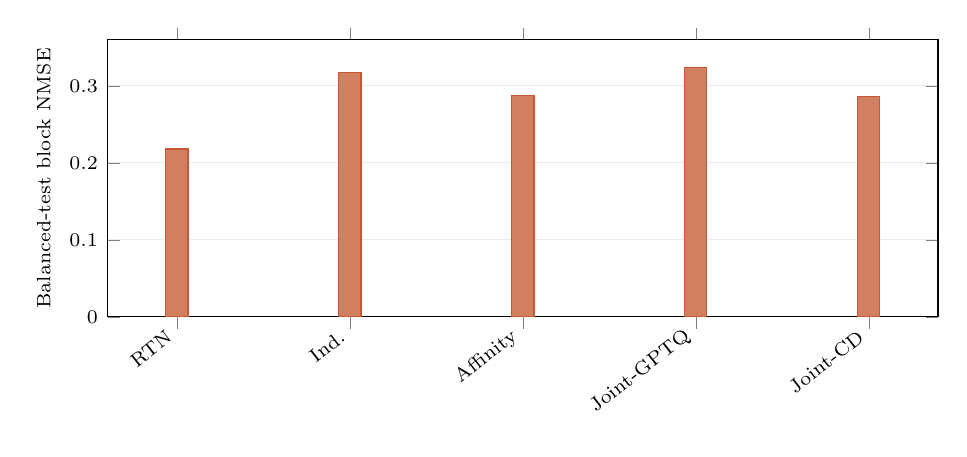
\begin{tikzpicture}
\begin{axis}[
  width=\linewidth,height=5.1cm,ybar,bar width=8pt,
  ymin=0,ymax=0.36,ymajorgrids=true,grid style={line!55},
  ylabel={Balanced-test block NMSE},
  symbolic x coords={RTN,Ind.,Affinity,Joint-GPTQ,Joint-CD},
  xtick=data,xticklabel style={rotate=38,anchor=east,font=\scriptsize},
  label style={font=\scriptsize},tick label style={font=\scriptsize}
]
\addplot[fill=rust!78,draw=rust] coordinates {
  (RTN,0.218108) (Ind.,0.317627) (Affinity,0.287923)
  (Joint-GPTQ,0.323935) (Joint-CD,0.286701)};
\end{axis}
\end{tikzpicture}
\end{minipage}\hfill
\begin{minipage}{0.48\textwidth}
\centering
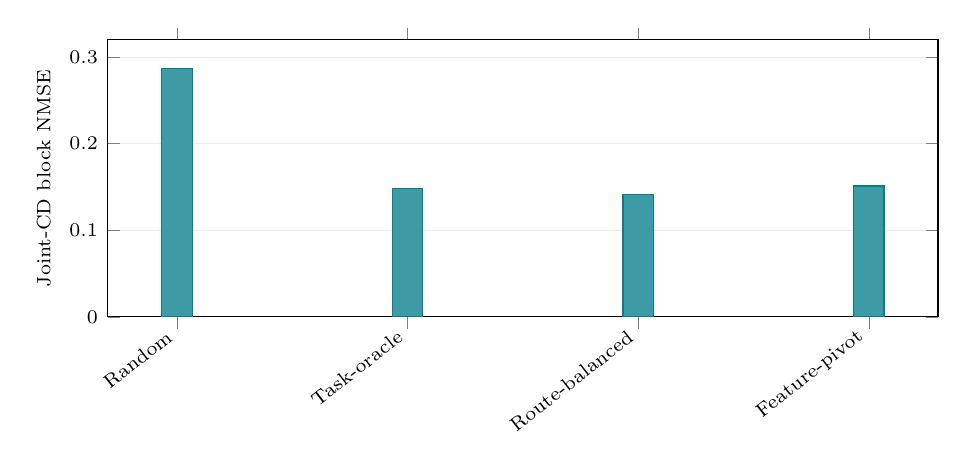
\begin{tikzpicture}
\begin{axis}[
  width=\linewidth,height=5.1cm,ybar,bar width=11pt,
  ymin=0,ymax=0.32,ymajorgrids=true,grid style={line!55},
  ylabel={Joint-CD block NMSE},
  symbolic x coords={Random,Task-oracle,Route-balanced,Feature-pivot},
  xtick=data,xticklabel style={rotate=38,anchor=east,font=\scriptsize},
  label style={font=\scriptsize},tick label style={font=\scriptsize}
]
\addplot[fill=teal!78,draw=teal] coordinates {
  (Random,0.286701) (Task-oracle,0.148036)
  (Route-balanced,0.141737) (Feature-pivot,0.151030)};
\end{axis}
\end{tikzpicture}
\end{minipage}
\caption{Left: balanced-test method comparison under random calibration, deliberately exposing distribution shift. Right: calibration-selector comparison for the fixed joint-coordinate method.}
\end{figure}

\subsection{Interpretation}

The toy evidence supports three statements and no more:
\begin{enumerate}
  \item Cross-expert terms create a real discrete optimization gain in a controlled MoE.
  \item A solver initialized from an independent result can realize most of the tiny exact-oracle gain while preserving a calibration no-worse guarantee.
  \item Held-out transfer requires calibration coverage of co-routing structure; random perplexity-style samples are not automatically sufficient.
\end{enumerate}

It does not establish a gain on a pretrained language model, activation quantization, all expert projections, or autoregressive task success.

\section{Most feasible real-model verification}

The next experiment should remain small and diagnostic.

\begin{enumerate}
  \item Select one open MoE with roughly 1B active parameters and expose one or a few MoE layers.  Quantize only expert down projections first, leaving attention, routers, shared experts, and the suffix in FP16.
  \item Cache 128--512 sequences but cap the number of gate-weighted activation rows per layer.  Run both random and route-signature-stratified subsets with identical token budgets.
  \item On a small channel slice, compute an exhaustive or beam-search joint oracle.  On the full selected layer, run the dense joint coordinate solver.  Do not add grouping or low-rank Hessian approximations.
  \item Compare RTN, independent GPTQ, affinity GPTQ, dense joint GPTQ, and baseline-initialized joint correction.  Report calibration and held-out aggregated block error, logits KL after the FP16 suffix, PPL, route-margin buckets, and the next-router Top-$k$ overlap.
  \item Repeat over at least three layers and five calibration seeds.  Separate tokens by co-routing edge frequency and router margin; an average alone can hide the mechanism.
\end{enumerate}

\begin{center}
\fcolorbox{rust}{rust!5}{\begin{minipage}{0.91\textwidth}
\textbf{Go / No-Go criterion.} Continue to Hessian acceleration only if (i) the small-slice exact joint oracle consistently improves over the exact independent solution, and (ii) dense baseline-initialized joint correction transfers a material fraction of that gain to held-out aggregated block error and at least one suffix metric.  If either condition fails, route correction and specialized calibration data should not be added to the core method.
\end{minipage}}
\end{center}

\section{Deferred acceleration}

If the dense verifier passes, the full Hessian can be approximated in a second paper stage.  Candidate structures include:
\begin{itemize}
  \item channel slices with complete cross-expert blocks inside each slice;
  \item expert groups induced by the co-routing graph;
  \item a block-sparse local term plus a low-rank global residual;
  \item Woodbury or iterative solves without materializing the full inverse.
\end{itemize}

Sparse-plus-low-rank decomposition and ADMM are relevant here, but not to the first-stage proof.  Introducing them earlier would confound modeling gain with approximation error.  The appropriate second-stage comparison is a Pareto curve against the dense oracle: Hessian storage, solve time, and retained joint-objective gain.

\section{Reproducibility}

The implementation requires PyTorch; Matplotlib is optional for standalone PNG summaries.  From the repository root:
\begin{verbatim}
.venv/bin/python moejointquant.py --self-test
.venv/bin/python moejointquant.py \
  --output hsvdquant/toy/results/moejointquant \
  --seeds 0 1 2 3 4
\end{verbatim}

The output directory always contains \texttt{results.json}, \texttt{metrics.csv}, and a Markdown report; PNG summaries are added when Matplotlib is available.  The JSON records all configuration values, every per-seed metric, exact-oracle checks, coordinate histories, and runtime.  The plots in this note are rendered directly from those reported means.

\section{Conclusion}

The most defensible core is not ``trajectory correction'' and not ``a faster MoE Hessian.''  It is the exact observation that co-routed experts form one weighted operator, together with a baseline-preserving discrete correction on that operator.  The global joint model has a simple dominance theorem; the executable solver has a monotonic calibration guarantee; and the suffix and router analyses state the additional conditions needed for local error to propagate safely.  The toy study is positive but also shows why calibration must be evaluated separately.  This provides a clean sequence for the paper: prove and verify joint gain first, then approximate its structure, and only then study route-aware calibration selection.

\begin{thebibliography}{9}
\small
\bibitem{gptq}
E. Frantar, S. Ashkboos, T. Hoefler, and D. Alistarh.
\newblock GPTQ: Accurate Post-Training Quantization for Generative Pre-trained Transformers.
\newblock \emph{ICLR}, 2023.

\bibitem{moequant}
Z. Chen et al.
\newblock MoEQuant: Enhancing Quantization for Mixture-of-Experts Large Language Models via Expert-Balanced Sampling and Affinity Guidance.
\newblock \emph{ICML}, 2025.

\bibitem{adm}
X. Yuan and J. Yang.
\newblock Sparse and Low-Rank Matrix Decomposition via Alternating Direction Methods.
\newblock 2011.
\end{thebibliography}

\end{document}
